% !TeX spellcheck = en_US
\documentclass[11pt]{extarticle}

\usepackage{graphicx,tikz,pgfplots,float,hyperref,cleveref}
\usetikzlibrary{calc,positioning,arrows,backgrounds,shapes.geometric}
\tikzset{background rectangle/.style={fill=black!10}, show background rectangle}
\pgfplotsset{compat=1.17}

% Split at comas for long formulas
\newcommand{\splitatcommas}[1]{%
	\begingroup
	\ifnum\mathcode`,="8000
	\else
	\begingroup\lccode`~=`, \lowercase{\endgroup
		\edef~{\mathchar\the\mathcode`, \penalty0 \noexpand\hspace{0pt plus 1em}}%
	}\mathcode`,="8000
	\fi
	#1%
	\endgroup
}

\begin{document}
	\begin{figure}[!h]
	\centering\includegraphics[width=\columnwidth]{../../../../website/src/main/jbake/assets/images/MessageVortexLogo_huge}
	\caption{The project logo}
	\label{fig:logo}
	\end{figure}
	Figure \ref{fig:logo} whows the project logo (should not be changed but maybe to be used to denote nodes as in \cref{fig:reducedMessageGraphPaths})
	
	\section{Part 3}
	\begin{figure}[!h]
		\centering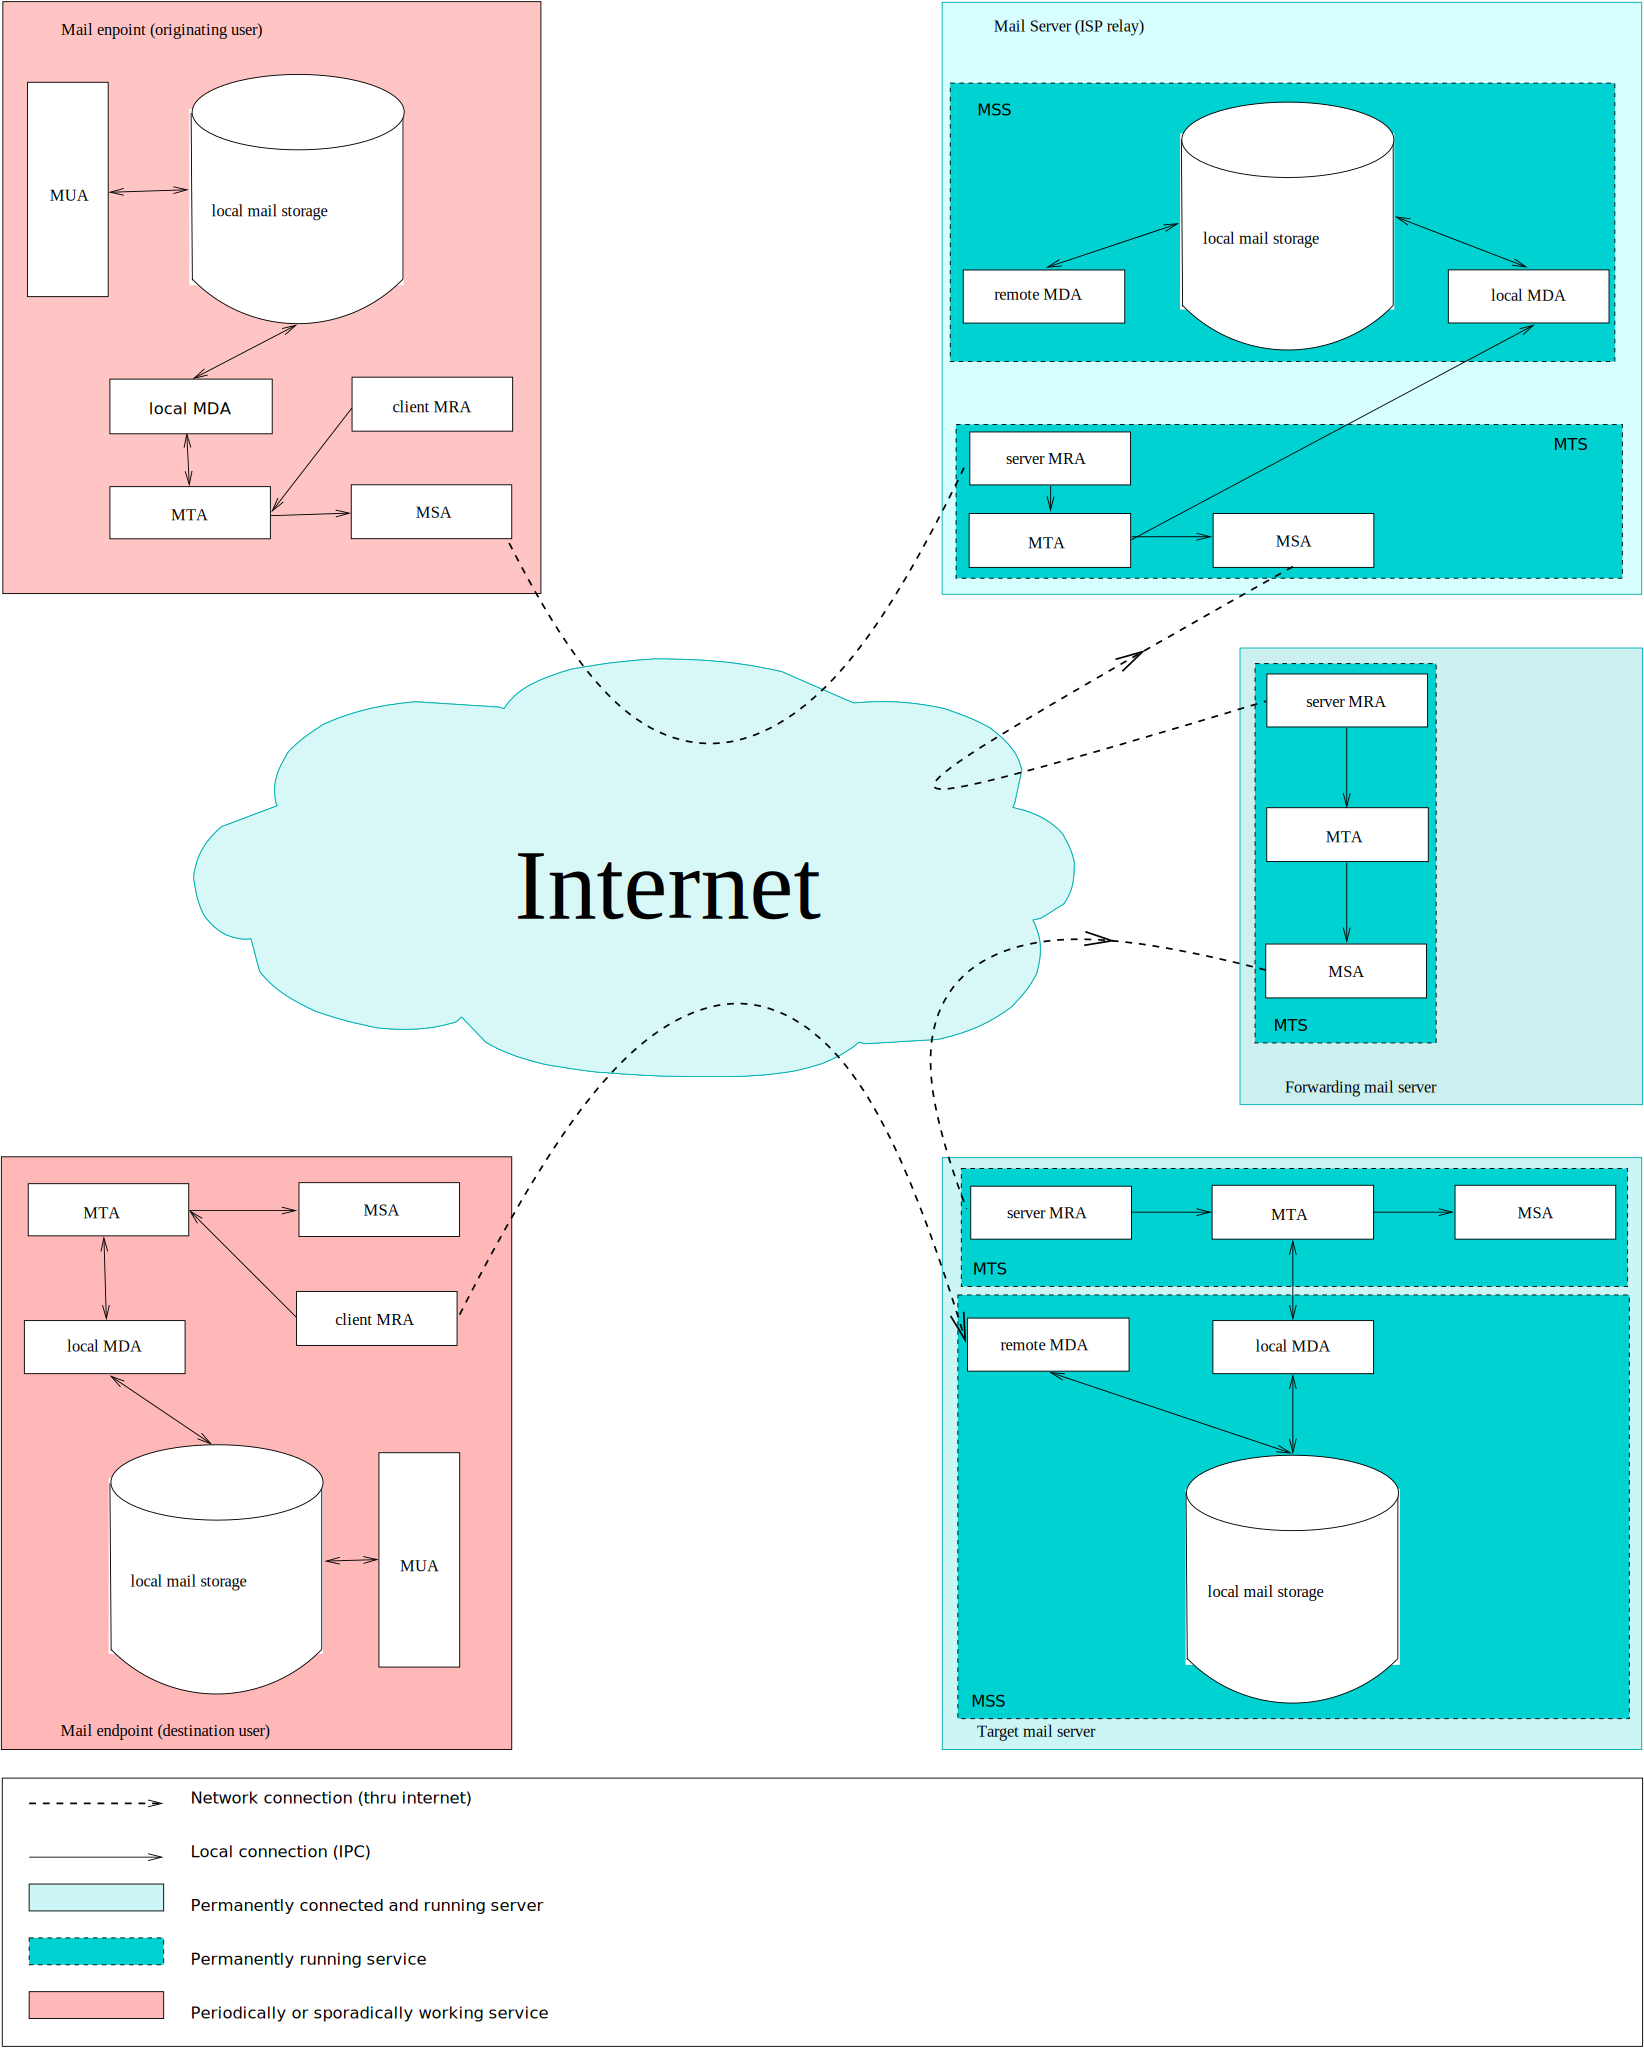
\includegraphics[width=\columnwidth]{inc/MailAgents1.pdf}
		\caption{Mail Agents}
		\label{fig:MailAgents}
	\end{figure}
	This \cref{fig:MailAgents} is at the beginning of part 3. It shows the relevant services of a mail router in a modified way. The figure fits the current style (which is considered bad). This graphic is however a single graphic.
	
	\section{Part 4}
	
	\begin{figure}[!h]\centering
		\includegraphics[width=0.8\columnwidth]{inc/addRedundancyOp}
		\caption{Outline of the addRedundancy operation}
		\label{fig:addRedundancyOperation}
	\end{figure}
	This \cref{fig:addRedundancyOperation} describes a core operation. It first takes an input vector, pads and splits it into a series of blocks, then applies an operation on it, and then executes an unpadded, symmetric encryption operation. This is one of the operations which is part in one of the subsequent graphics. It would be good if this operation looks somehow similar.
	 
	\begin{figure}[!h]
	 	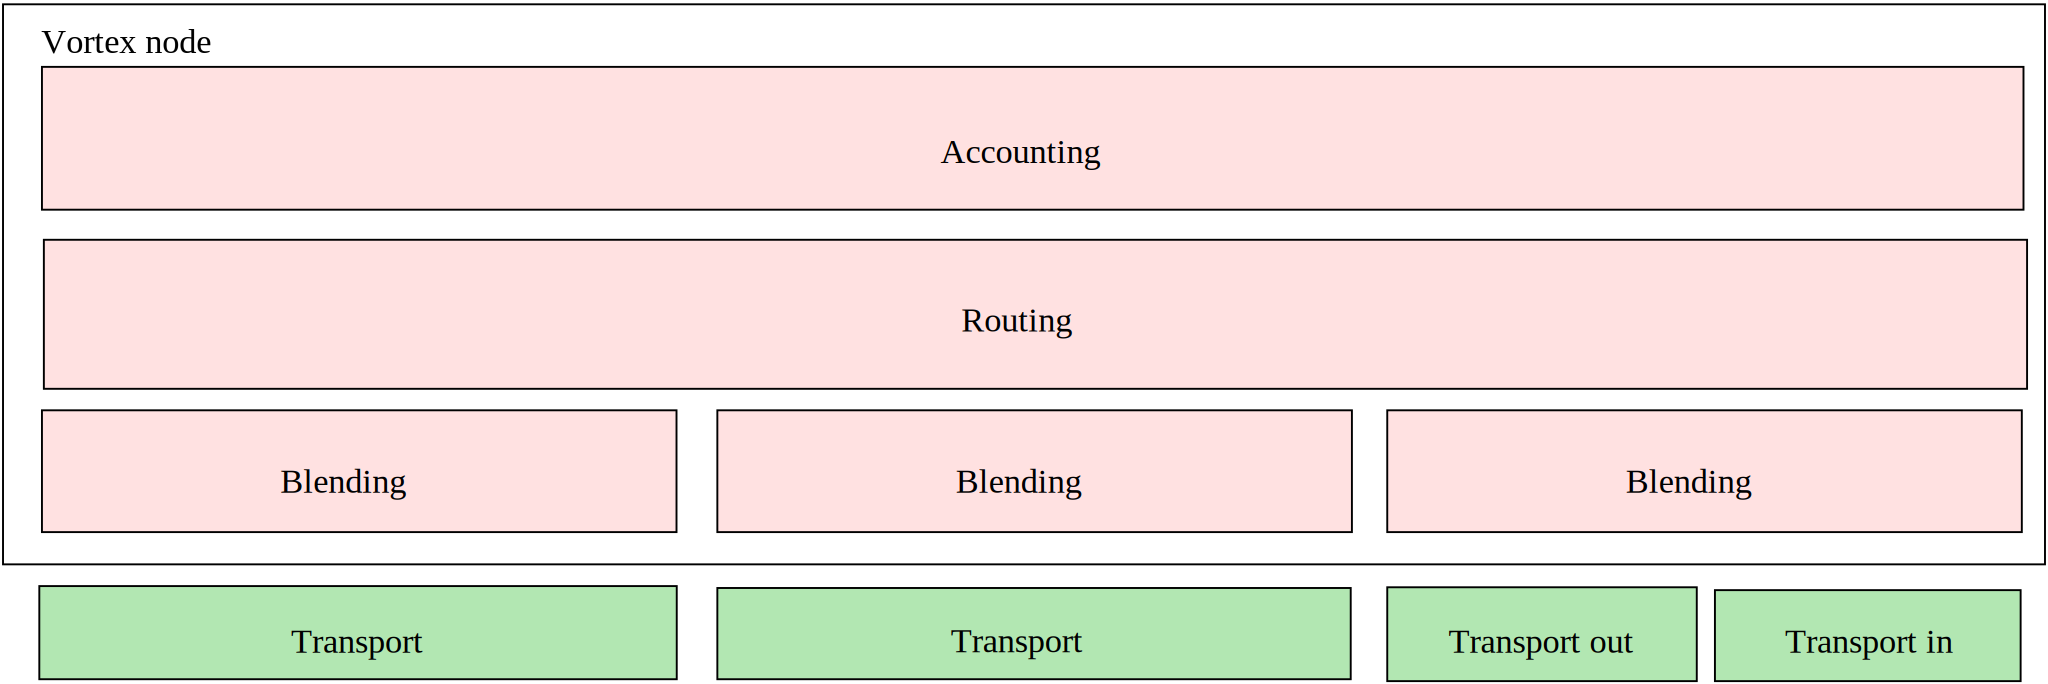
\includegraphics[width=\textwidth]{inc/layerDesign}
	 	\caption{The protocol layers}
	 	\label{fig:protocolLayers}
	\end{figure}
	This \cref{fig:protocolLayers} shows the protocol layers. Important: The transport layer is not part of the Protocol. The coloring overlaps senslessly  with \cref{fig:addRedundancyOperation}.
	 
	\begin{figure}[!h]
	 	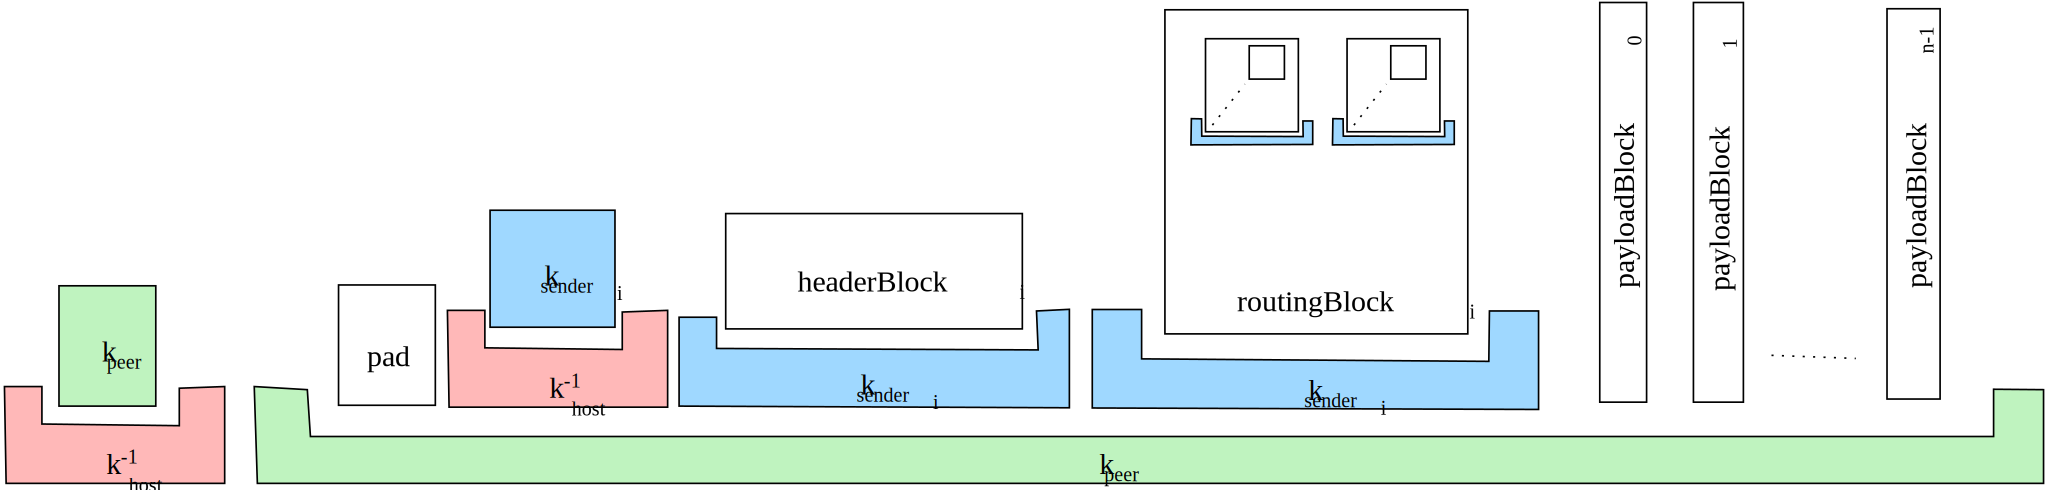
\includegraphics[width=\textwidth]{inc/blockLayoutSimplified}
	 	$\splitatcommas{\langle \mathbf{MPREFIX_o}, E_{K_{peer_{o+1}}}\left( \mathbf{HPREFIX_o}, \mathbf{HEADER_o}^{K_{sender_o}}, \mathbf{ROUTING_o}^{K_{sender_o}}, payload* \right) \rangle}$
	 	\caption{Simplified message outline visually and in math}
	 	\label{fig:messageOutline}
	\end{figure}
	This \cref{fig:messageOutline} shows a simplified block layout of a Vortex message. The colors denote different encryption keys and the underlying braces encrypted section (some are doubly encrypted). Symmetric and asymmetric encryption is only denoted in the texts. The math at the bottom is badly aligned.
	 
	\begin{figure}[H]
	 	\centering
	 	\includegraphics[height=0.45\textheight]{inc/flowchart_message_receiving}
	 	\caption{flow diagram showing processing of outgoing messages}
	 	\label{fig:msgReceiveProcessing}
	\end{figure}
 
 	\begin{figure}[H]
 		\centering
 		\includegraphics[height=0.40\textheight]{inc/flowchart_message_sending}
 		\caption{flow diagram showing processing of outgoing messages}
 		\label{fig:msgSendProcessing}
 	\end{figure}
	The flowchart in \cref{fig:msgReceiveProcessing} and \cref{fig:msgSendProcessing} of message processing looks somehow out of place as they were done in visio (and they are too small).
 	
 	
 	\section{Part 6}
	 \begin{figure}[H]\centering\resizebox{.95\linewidth}{!}{
	 		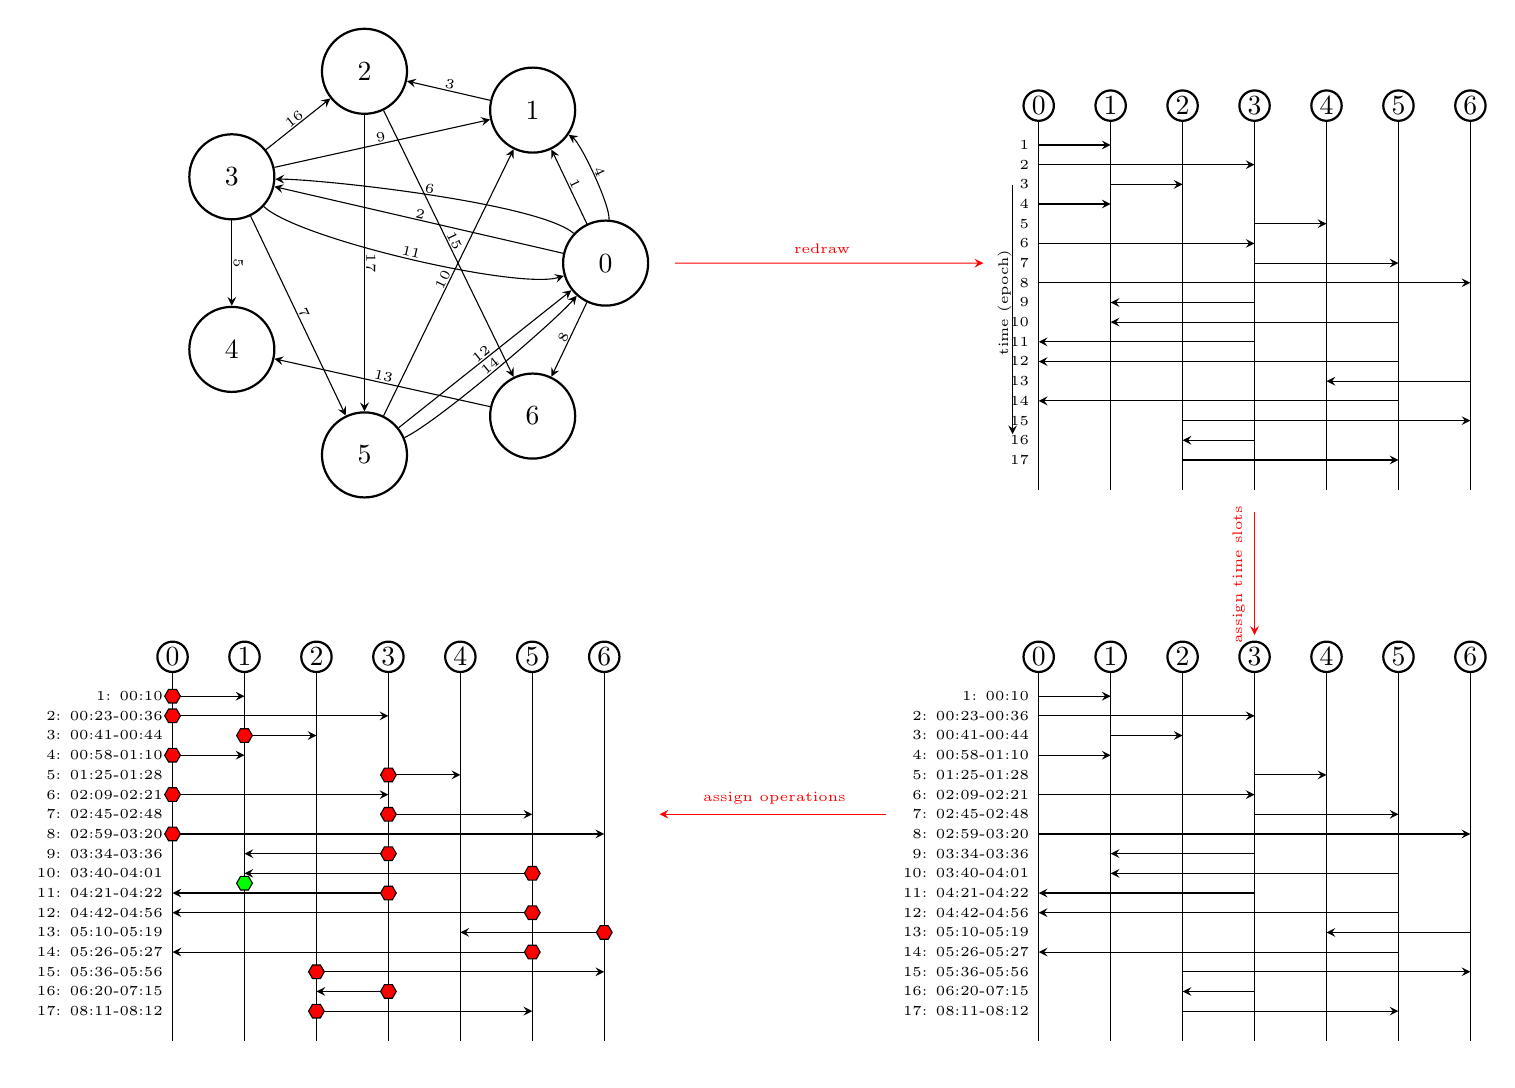
\begin{tikzpicture}[node distance=0.5cm,auto,>=stealth]
	 			\begin{scope}[baseline=(current bounding box.center),xshift=-3cm]
	 				\tikzstyle{knode}=[circle,draw=black,thick,inner sep=8pt,baseline=(current bounding box.center)]
	 				\node[knode] (r0) at (0:2.5cm) {0};
	 				\node[knode] (r1) at (51:2.5cm) {1};
	 				\node[knode] (r2) at (103:2.5cm) {2};
	 				\node[knode] (r3) at (154:2.5cm) {3};
	 				\node[knode] (r4) at (206:2.5cm) {4};
	 				\node[knode] (r5) at (257:2.5cm) {5};
	 				\node[knode] (r6) at (309:2.5cm) {6};
	 				%arrows
	 				\draw[->] (r0)--node[sloped, anchor=center, above=-1mm]{\tiny 1}(r1);
	 				\draw[->] (r0)--node[sloped, anchor=center, above=-1mm]{\tiny 2}(r3);
	 				\draw[->] (r1)--node[sloped, anchor=center, above=-1mm]{\tiny 3}(r2);
	 				\draw[->,bend right,looseness=0.4] (r0) edge node[sloped, anchor=center, above=-1mm]{\tiny 4} (r1);
	 				\draw[->] (r3)-- node[sloped, anchor=center, above=-1mm]{\tiny 5}(r4);
	 				\draw[->,bend right,looseness=0.4,in=190] (r0) edge  node[sloped, anchor=center, above=-1mm]{\tiny 6}(r3);
	 				\draw[->] (r3)-- node[sloped, anchor=center, above=-1mm]{\tiny 7}(r5);
	 				\draw[->] (r0)-- node[sloped, anchor=center, above=-1mm]{\tiny 8}(r6);
	 				\draw[->] (r3)-- node[sloped, anchor=center, above=-1mm]{\tiny 9}(r1);
	 				\draw[->] (r5)-- node[sloped, anchor=center, above=-1mm]{\tiny 10}(r1);
	 				\draw[->,bend right,looseness=0.4] (r3)edge node[sloped, anchor=center, above=-1mm]{\tiny 11}(r0);
	 				\draw[->] (r5)-- node[sloped, anchor=center, above=-1mm]{\tiny 12}(r0);
	 				\draw[->] (r6)-- node[sloped, anchor=center, above=-1mm]{\tiny 13}(r4);
	 				\draw[->,bend right,looseness=0.4,out=-15,in=190] (r5) edge  node[sloped, anchor=center, above=-1mm]{\tiny 14}(r0);
	 				\draw[->] (r2)-- node[sloped, anchor=center, above=-1mm]{\tiny 15}(r6);
	 				\draw[->] (r3)-- node[sloped, anchor=center, above=-1mm]{\tiny 16}(r2);
	 				\draw[->] (r2)-- node[sloped, anchor=center, above=-1mm]{\tiny 17}(r5);
	 			\end{scope}
	 			\begin{scope}[baseline=(current bounding box.center),xshift=5cm,yshift=2cm]
	 				\tikzstyle{knode}=[circle,draw=black,thick,inner sep=1pt,baseline=(current bounding box.center)]
	 				\node[knode] (n0) {0};
	 				\node[knode,right = of n0] (n1) {1};
	 				\node[knode,right = of n1] (n2) {2};
	 				\node[knode,right = of n2] (n3) {3};
	 				\node[knode,right = of n3] (n4) {4};
	 				\node[knode,right = of n4] (n5) {5};
	 				\node[knode,right = of n5] (n6) {6};
	 				\node[left = 0mm of n0] (nm0) {};
	 				\node[below of=n0, node distance=5cm] (n0Ground) {};
	 				\node[below of=n1, node distance=5cm] (n1Ground) {};
	 				\node[below of=n2, node distance=5cm] (n2Ground) {};
	 				\node[below of=n3, node distance=5cm] (n3Ground) {};
	 				\node[below of=n4, node distance=5cm] (n4Ground) {};
	 				\node[below of=n5, node distance=5cm] (n5Ground) {};
	 				\node[below of=n6, node distance=5cm] (n6Ground) {};
	 				\node[below of=nm0,node distance=5cm] (nm0Ground) {};
	 				% lines down
	 				\draw (n0) -- (n0Ground);
	 				\draw (n1) -- (n1Ground);
	 				\draw (n2) -- (n2Ground);
	 				\draw (n3) -- (n3Ground);
	 				\draw (n4) -- (n4Ground);
	 				\draw (n5) -- (n5Ground);
	 				\draw (n6) -- (n6Ground);
	 				%arrows
	 				\draw[->] ($(n0)!0.10!(n0Ground)$)--($(n1)!0.10!(n1Ground)$);\node[anchor=east] at ($(n0)!0.10!(n0Ground)$) {\tiny 1};
	 				\draw[->] ($(n0)!0.15!(n0Ground)$)--($(n3)!0.15!(n3Ground)$);\node[anchor=east] at ($(n0)!0.15!(n0Ground)$) {\tiny 2};
	 				\draw[->] ($(n1)!0.20!(n1Ground)$)--($(n2)!0.20!(n2Ground)$);\node[anchor=east] at ($(n0)!0.20!(n0Ground)$) {\tiny 3};
	 				\draw[->] ($(n0)!0.25!(n0Ground)$)--($(n1)!0.25!(n1Ground)$);\node[anchor=east] at ($(n0)!0.25!(n0Ground)$) {\tiny 4};
	 				\draw[->] ($(n3)!0.30!(n3Ground)$)--($(n4)!0.30!(n4Ground)$);\node[anchor=east] at ($(n0)!0.30!(n0Ground)$) {\tiny 5};
	 				\draw[->] ($(n0)!0.35!(n0Ground)$)--($(n3)!0.35!(n3Ground)$);\node[anchor=east] at ($(n0)!0.35!(n0Ground)$) {\tiny 6};
	 				\draw[->] ($(n3)!0.40!(n3Ground)$)--($(n5)!0.40!(n5Ground)$);\node[anchor=east] at ($(n0)!0.40!(n0Ground)$) {\tiny 7};
	 				\draw[->] ($(n0)!0.45!(n0Ground)$)--($(n6)!0.45!(n6Ground)$);\node[anchor=east] at ($(n0)!0.45!(n0Ground)$) {\tiny 8};
	 				\draw[->] ($(n3)!0.50!(n3Ground)$)--($(n1)!0.50!(n1Ground)$);\node[anchor=east] at ($(n0)!0.50!(n0Ground)$) {\tiny 9};
	 				\draw[->] ($(n5)!0.55!(n5Ground)$)--($(n1)!0.55!(n1Ground)$);\node[anchor=east] at ($(n0)!0.55!(n0Ground)$) {\tiny 10};
	 				\draw[->] ($(n3)!0.60!(n3Ground)$)--($(n0)!0.60!(n0Ground)$);\node[anchor=east] at ($(n0)!0.60!(n0Ground)$) {\tiny 11};
	 				\draw[->] ($(n5)!0.65!(n5Ground)$)--($(n0)!0.65!(n0Ground)$);\node[anchor=east] at ($(n0)!0.65!(n0Ground)$) {\tiny 12};
	 				\draw[->] ($(n6)!0.70!(n6Ground)$)--($(n4)!0.70!(n4Ground)$);\node[anchor=east] at ($(n0)!0.70!(n0Ground)$) {\tiny 13};
	 				\draw[->] ($(n5)!0.75!(n5Ground)$)--($(n0)!0.75!(n0Ground)$);\node[anchor=east] at ($(n0)!0.75!(n0Ground)$) {\tiny 14};
	 				\draw[->] ($(n2)!0.80!(n2Ground)$)--($(n6)!0.80!(n6Ground)$);\node[anchor=east] at ($(n0)!0.80!(n0Ground)$) {\tiny 15};
	 				\draw[->] ($(n3)!0.85!(n3Ground)$)--($(n2)!0.85!(n2Ground)$);\node[anchor=east] at ($(n0)!0.85!(n0Ground)$) {\tiny 16};
	 				\draw[->] ($(n2)!0.90!(n2Ground)$)--($(n5)!0.90!(n5Ground)$);\node[anchor=east] at ($(n0)!0.90!(n0Ground)$) {\tiny 17};
	 				% Legend
	 				\draw[->,shorten <=25pt,shorten >=20pt] (nm0) --node[above=-1mm,sloped,anchor=center,rotate=180] {$\textrm{\tiny time (epoch)}$} (nm0Ground)  ;
	 				
	 			\end{scope}
	 			\draw[->,shorten <=25pt,shorten >=20pt,draw=red] ($(r0)!0.0!(r0)$)--node[above,sloped]{\tiny \textcolor{red}{redraw}}($(n0)!0.4!(n0Ground)$);
	 			\begin{scope}[baseline=(current bounding box.center),xshift=5cm,yshift=-5cm]
	 				\tikzstyle{knode}=[circle,draw=black,thick,inner sep=1pt,baseline=(current bounding box.center)]
	 				\node[knode] (n10) {0};
	 				\node[knode,right = of n10] (n11) {1};
	 				\node[knode,right = of n11] (n12) {2};
	 				\node[knode,right = of n12] (n13) {3};
	 				\node[knode,right = of n13] (n14) {4};
	 				\node[knode,right = of n14] (n15) {5};
	 				\node[knode,right = of n15] (n16) {6};
	 				\node[left = 0mm of n10] (nm10) {};
	 				\node[below of=n10, node distance=5cm] (n10Ground) {};
	 				\node[below of=n11, node distance=5cm] (n11Ground) {};
	 				\node[below of=n12, node distance=5cm] (n12Ground) {};
	 				\node[below of=n13, node distance=5cm] (n13Ground) {};
	 				\node[below of=n14, node distance=5cm] (n14Ground) {};
	 				\node[below of=n15, node distance=5cm] (n15Ground) {};
	 				\node[below of=n16, node distance=5cm] (n16Ground) {};
	 				\node[below of=nm10,node distance=5cm] (nm10Ground) {};
	 				% lines down
	 				\draw (n10) -- (n10Ground);
	 				\draw (n11) -- (n11Ground);
	 				\draw (n12) -- (n12Ground);
	 				\draw (n13) -- (n13Ground);
	 				\draw (n14) -- (n14Ground);
	 				\draw (n15) -- (n15Ground);
	 				\draw (n16) -- (n16Ground);
	 				%arrows
	 				\draw[->] ($(n10)!0.10!(n10Ground)$)--($(n11)!0.10!(n11Ground)$);\node[anchor=east] at ($(n10)!0.10!(n10Ground)$) {\tiny 1: 00:10};
	 				\draw[->] ($(n10)!0.15!(n10Ground)$)--($(n13)!0.15!(n13Ground)$);\node[anchor=east] at ($(n10)!0.15!(n10Ground)$) {\tiny 2: 00:23-00:36};
	 				\draw[->] ($(n11)!0.20!(n11Ground)$)--($(n12)!0.20!(n12Ground)$);\node[anchor=east] at ($(n10)!0.20!(n10Ground)$) {\tiny 3: 00:41-00:44};
	 				\draw[->] ($(n10)!0.25!(n10Ground)$)--($(n11)!0.25!(n11Ground)$);\node[anchor=east] at ($(n10)!0.25!(n10Ground)$) {\tiny 4: 00:58-01:10};
	 				\draw[->] ($(n13)!0.30!(n13Ground)$)--($(n14)!0.30!(n14Ground)$);\node[anchor=east] at ($(n10)!0.30!(n10Ground)$) {\tiny 5: 01:25-01:28};
	 				\draw[->] ($(n10)!0.35!(n10Ground)$)--($(n13)!0.35!(n13Ground)$);\node[anchor=east] at ($(n10)!0.35!(n10Ground)$) {\tiny 6: 02:09-02:21};
	 				\draw[->] ($(n13)!0.40!(n13Ground)$)--($(n15)!0.40!(n15Ground)$);\node[anchor=east] at ($(n10)!0.40!(n10Ground)$) {\tiny 7: 02:45-02:48};
	 				\draw[->] ($(n10)!0.45!(n10Ground)$)--($(n16)!0.45!(n16Ground)$);\node[anchor=east] at ($(n10)!0.45!(n10Ground)$) {\tiny 8: 02:59-03:20};
	 				\draw[->] ($(n13)!0.50!(n13Ground)$)--($(n11)!0.50!(n11Ground)$);\node[anchor=east] at ($(n10)!0.50!(n10Ground)$) {\tiny 9: 03:34-03:36};
	 				\draw[->] ($(n15)!0.55!(n15Ground)$)--($(n11)!0.55!(n11Ground)$);\node[anchor=east] at ($(n10)!0.55!(n10Ground)$) {\tiny 10: 03:40-04:01};
	 				\draw[->] ($(n13)!0.60!(n13Ground)$)--($(n10)!0.60!(n10Ground)$);\node[anchor=east] at ($(n10)!0.60!(n10Ground)$) {\tiny 11: 04:21-04:22};
	 				\draw[->] ($(n15)!0.65!(n15Ground)$)--($(n10)!0.65!(n10Ground)$);\node[anchor=east] at ($(n10)!0.65!(n10Ground)$) {\tiny 12: 04:42-04:56};
	 				\draw[->] ($(n16)!0.70!(n16Ground)$)--($(n14)!0.70!(n14Ground)$);\node[anchor=east] at ($(n10)!0.70!(n10Ground)$) {\tiny 13: 05:10-05:19};
	 				\draw[->] ($(n15)!0.75!(n15Ground)$)--($(n10)!0.75!(n10Ground)$);\node[anchor=east] at ($(n10)!0.75!(n10Ground)$) {\tiny 14: 05:26-05:27};
	 				\draw[->] ($(n12)!0.80!(n12Ground)$)--($(n16)!0.80!(n16Ground)$);\node[anchor=east] at ($(n10)!0.80!(n10Ground)$) {\tiny 15: 05:36-05:56};
	 				\draw[->] ($(n13)!0.85!(n13Ground)$)--($(n12)!0.85!(n12Ground)$);\node[anchor=east] at ($(n10)!0.85!(n10Ground)$) {\tiny 16: 06:20-07:15};
	 				\draw[->] ($(n12)!0.90!(n12Ground)$)--($(n15)!0.90!(n15Ground)$);\node[anchor=east] at ($(n10)!0.90!(n10Ground)$) {\tiny 17: 08:11-08:12};
	 			\end{scope}
	 			\draw[->,shorten <=1pt,shorten >=2pt,draw=red] (n3Ground)--node[rotate=180,above,sloped]{\tiny \textcolor{red}{assign time slots}}(n13);
	 			\begin{scope}[baseline=(current bounding box.center),xshift=-6cm,yshift=-5cm]
	 				\tikzstyle{knode}=[circle,draw=black,thick,inner sep=1pt,baseline=(current bounding box.center)]
	 				\node[knode] (n20) {0};
	 				\node[knode,right = of n20] (n21) {1};
	 				\node[knode,right = of n21] (n22) {2};
	 				\node[knode,right = of n22] (n23) {3};
	 				\node[knode,right = of n23] (n24) {4};
	 				\node[knode,right = of n24] (n25) {5};
	 				\node[knode,right = of n25] (n26) {6};
	 				\node[left = 0mm of n20] (nm20) {};
	 				\node[below of=n20, node distance=5cm] (n20Ground) {};
	 				\node[below of=n21, node distance=5cm] (n21Ground) {};
	 				\node[below of=n22, node distance=5cm] (n22Ground) {};
	 				\node[below of=n23, node distance=5cm] (n23Ground) {};
	 				\node[below of=n24, node distance=5cm] (n24Ground) {};
	 				\node[below of=n25, node distance=5cm] (n25Ground) {};
	 				\node[below of=n26, node distance=5cm] (n26Ground) {};
	 				\node[below of=nm20,node distance=5cm] (nm20Ground) {};
	 				% lines down
	 				\draw (n20) -- (n20Ground);
	 				\draw (n21) -- (n21Ground);
	 				\draw (n22) -- (n22Ground);
	 				\draw (n23) -- (n23Ground);
	 				\draw (n24) -- (n24Ground);
	 				\draw (n25) -- (n25Ground);
	 				\draw (n26) -- (n26Ground);
	 				%arrows
	 				\draw[->] ($(n20)!0.10!(n20Ground)$)--($(n21)!0.10!(n21Ground)$);\node[anchor=east] at ($(n20)!0.10!(n20Ground)$) {\tiny 1: 00:10}; \node[regular polygon,regular polygon sides=6,draw,fill=red,inner sep=0mm,minimum size=2mm]  at ($(n20)!0.10!(n20Ground)$) {};
	 				\draw[->] ($(n20)!0.15!(n20Ground)$)--($(n23)!0.15!(n23Ground)$);\node[anchor=east] at ($(n20)!0.15!(n20Ground)$) {\tiny 2: 00:23-00:36};\node[regular polygon,regular polygon sides=6,draw,fill=red,inner sep=0mm,minimum size=2mm]  at ($(n20)!0.15!(n20Ground)$) {};
	 				\draw[->] ($(n21)!0.20!(n21Ground)$)--($(n22)!0.20!(n22Ground)$);\node[anchor=east] at ($(n20)!0.20!(n20Ground)$) {\tiny 3: 00:41-00:44};\node[regular polygon,regular polygon sides=6,draw,fill=red,inner sep=0mm,minimum size=2mm]  at ($(n21)!0.20!(n21Ground)$) {};
	 				\draw[->] ($(n20)!0.25!(n20Ground)$)--($(n21)!0.25!(n21Ground)$);\node[anchor=east] at ($(n20)!0.25!(n20Ground)$) {\tiny 4: 00:58-01:10};\node[regular polygon,regular polygon sides=6,draw,fill=red,inner sep=0mm,minimum size=2mm]  at ($(n20)!0.25!(n20Ground)$) {};
	 				\draw[->] ($(n23)!0.30!(n23Ground)$)--($(n24)!0.30!(n24Ground)$);\node[anchor=east] at ($(n20)!0.30!(n20Ground)$) {\tiny 5: 01:25-01:28};\node[regular polygon,regular polygon sides=6,draw,fill=red,inner sep=0mm,minimum size=2mm]  at ($(n23)!0.30!(n23Ground)$) {};
	 				\draw[->] ($(n20)!0.35!(n20Ground)$)--($(n23)!0.35!(n23Ground)$);\node[anchor=east] at ($(n20)!0.35!(n20Ground)$) {\tiny 6: 02:09-02:21};\node[regular polygon,regular polygon sides=6,draw,fill=red,inner sep=0mm,minimum size=2mm]  at ($(n20)!0.35!(n20Ground)$) {};
	 				\draw[->] ($(n23)!0.40!(n23Ground)$)--($(n25)!0.40!(n25Ground)$);\node[anchor=east] at ($(n20)!0.40!(n20Ground)$) {\tiny 7: 02:45-02:48};\node[regular polygon,regular polygon sides=6,draw,fill=red,inner sep=0mm,minimum size=2mm]  at ($(n23)!0.40!(n23Ground)$) {};
	 				\draw[->] ($(n20)!0.45!(n20Ground)$)--($(n26)!0.45!(n26Ground)$);\node[anchor=east] at ($(n20)!0.45!(n20Ground)$) {\tiny 8: 02:59-03:20};\node[regular polygon,regular polygon sides=6,draw,fill=red,inner sep=0mm,minimum size=2mm]  at ($(n20)!0.45!(n20Ground)$) {};
	 				\draw[->] ($(n23)!0.50!(n23Ground)$)--($(n21)!0.50!(n21Ground)$);\node[anchor=east] at ($(n20)!0.50!(n20Ground)$) {\tiny 9: 03:34-03:36};\node[regular polygon,regular polygon sides=6,draw,fill=red,inner sep=0mm,minimum size=2mm]  at ($(n23)!0.50!(n23Ground)$) {};
	 				\draw[->] ($(n25)!0.55!(n25Ground)$)--($(n21)!0.55!(n21Ground)$);\node[anchor=east] at ($(n20)!0.55!(n20Ground)$) {\tiny 10: 03:40-04:01};\node[regular polygon,regular polygon sides=6,draw,fill=red,inner sep=0mm,minimum size=2mm]  at ($(n25)!0.55!(n25Ground)$) {};
	 				\node[regular polygon,regular polygon sides=6,draw,fill=green,inner sep=0mm,minimum size=2mm]  at ($(n21)!0.575!(n21Ground)$) {}; %% reassembly node
	 				\draw[->] ($(n23)!0.60!(n23Ground)$)--($(n20)!0.60!(n20Ground)$);\node[anchor=east] at ($(n20)!0.60!(n20Ground)$) {\tiny 11: 04:21-04:22};\node[regular polygon,regular polygon sides=6,draw,fill=red,inner sep=0mm,minimum size=2mm]  at ($(n23)!0.60!(n23Ground)$) {};
	 				\draw[->] ($(n25)!0.65!(n25Ground)$)--($(n20)!0.65!(n20Ground)$);\node[anchor=east] at ($(n20)!0.65!(n20Ground)$) {\tiny 12: 04:42-04:56};\node[regular polygon,regular polygon sides=6,draw,fill=red,inner sep=0mm,minimum size=2mm]  at ($(n25)!0.65!(n25Ground)$) {};
	 				\draw[->] ($(n26)!0.70!(n26Ground)$)--($(n24)!0.70!(n24Ground)$);\node[anchor=east] at ($(n20)!0.70!(n20Ground)$) {\tiny 13: 05:10-05:19};\node[regular polygon,regular polygon sides=6,draw,fill=red,inner sep=0mm,minimum size=2mm]  at ($(n26)!0.70!(n26Ground)$) {};
	 				\draw[->] ($(n25)!0.75!(n25Ground)$)--($(n20)!0.75!(n20Ground)$);\node[anchor=east] at ($(n20)!0.75!(n20Ground)$) {\tiny 14: 05:26-05:27};\node[regular polygon,regular polygon sides=6,draw,fill=red,inner sep=0mm,minimum size=2mm]  at ($(n25)!0.75!(n25Ground)$) {};
	 				\draw[->] ($(n22)!0.80!(n22Ground)$)--($(n26)!0.80!(n26Ground)$);\node[anchor=east] at ($(n20)!0.80!(n20Ground)$) {\tiny 15: 05:36-05:56};\node[regular polygon,regular polygon sides=6,draw,fill=red,inner sep=0mm,minimum size=2mm]  at ($(n22)!0.80!(n22Ground)$) {};
	 				\draw[->] ($(n23)!0.85!(n23Ground)$)--($(n22)!0.85!(n22Ground)$);\node[anchor=east] at ($(n20)!0.85!(n20Ground)$) {\tiny 16: 06:20-07:15};\node[regular polygon,regular polygon sides=6,draw,fill=red,inner sep=0mm,minimum size=2mm]  at ($(n23)!0.85!(n23Ground)$) {};
	 				\draw[->] ($(n22)!0.90!(n22Ground)$)--($(n25)!0.90!(n25Ground)$);\node[anchor=east] at ($(n20)!0.90!(n20Ground)$) {\tiny 17: 08:11-08:12};\node[regular polygon,regular polygon sides=6,draw,fill=red,inner sep=0mm,minimum size=2mm]  at ($(n22)!0.90!(n22Ground)$) {};
	 			\end{scope}
	 			\draw[->,shorten <=55pt,shorten >=20pt,draw=red] ($(n10)!0.4!(n10Ground)$)--node[above,xshift=-17pt]{\tiny \textcolor{red}{assign operations}}($(n26)!0.4!(n26Ground)$);
	 		\end{tikzpicture}
	 	}
	 	\caption{Transformation of a graph into a sequence of messages}
	 	\label{fig:transformGraph}
	 \end{figure}
 	Figure \ref{fig:transformGraph} shows the full transformation of the graph. The Image is ok but looks  "simple".
 
 	 \begin{figure}[H]
 	 	\resizebox{.9\linewidth}{!}{
 	 		\begin{tikzpicture}[>=stealth',shorten <=0.5pt,
 	 			main/.style={draw,minimum width=0.5cm},child/.style={draw,minimum width=0.5cm}]		
 	 			\tikzstyle{level 1}=[sibling angle=25.71]
 	 			
 	 			\node[main] (a) {
 	 				\begin{tikzpicture}
 	 					\node[] (n0) {0};
 	 					\node[right = of n0] (n1) {1};
 	 					\node[right = of n1] (n2) {2};
 	 					\node[right = of n2] (n3) {3};
 	 					\node[right = of n3] (n4) {4};
 	 					\node[right = of n4] (n5) {5};
 	 					\node[right = of n5] (n6) {6};
 	 					\node[below of=n0, node distance=5cm] (n0Ground) {};
 	 					\node[below of=n1, node distance=5cm] (n1Ground) {};
 	 					\node[below of=n2, node distance=5cm] (n2Ground) {};
 	 					\node[below of=n3, node distance=5cm] (n3Ground) {};
 	 					\node[below of=n4, node distance=5cm] (n4Ground) {};
 	 					\node[below of=n5, node distance=5cm] (n5Ground) {};
 	 					\node[below of=n6, node distance=5cm] (n6Ground) {};
 	 					% lines down
 	 					\draw (n0) -- (n0Ground);
 	 					\draw (n1) -- (n1Ground);
 	 					\draw (n2) -- (n2Ground);
 	 					\draw (n3) -- (n3Ground);
 	 					\draw (n4) -- (n4Ground);
 	 					\draw (n5) -- (n5Ground);
 	 					\draw (n6) -- (n6Ground);
 	 					%arrows
 	 					\draw[->] ($(n0)!0.10!(n0Ground)$)--($(n1)!0.10!(n1Ground)$);
 	 					\draw[->] ($(n0)!0.15!(n0Ground)$)--($(n3)!0.15!(n3Ground)$);
 	 					\draw[->] ($(n1)!0.20!(n1Ground)$)--($(n2)!0.20!(n2Ground)$);
 	 					\draw[->] ($(n0)!0.25!(n0Ground)$)--($(n1)!0.25!(n1Ground)$);
 	 					\draw[->] ($(n3)!0.30!(n3Ground)$)--($(n4)!0.30!(n4Ground)$);
 	 					\draw[->] ($(n0)!0.35!(n0Ground)$)--($(n3)!0.35!(n3Ground)$);
 	 					\draw[->] ($(n3)!0.40!(n3Ground)$)--($(n5)!0.40!(n5Ground)$);
 	 					\draw[->] ($(n0)!0.45!(n0Ground)$)--($(n6)!0.45!(n6Ground)$);
 	 					\draw[->] ($(n3)!0.50!(n3Ground)$)--($(n1)!0.50!(n1Ground)$);
 	 					\draw[->] ($(n5)!0.55!(n5Ground)$)--($(n1)!0.55!(n1Ground)$);
 	 					\draw[->] ($(n3)!0.60!(n3Ground)$)--($(n0)!0.60!(n0Ground)$);
 	 					\draw[->] ($(n5)!0.65!(n5Ground)$)--($(n0)!0.65!(n0Ground)$);
 	 					\draw[->] ($(n6)!0.70!(n6Ground)$)--($(n4)!0.70!(n4Ground)$);
 	 					\draw[->] ($(n5)!0.75!(n5Ground)$)--($(n0)!0.75!(n0Ground)$);
 	 					\draw[->] ($(n2)!0.80!(n2Ground)$)--($(n6)!0.80!(n6Ground)$);
 	 					\draw[->] ($(n3)!0.85!(n3Ground)$)--($(n2)!0.85!(n2Ground)$);
 	 					\draw[->] ($(n2)!0.90!(n2Ground)$)--($(n5)!0.90!(n5Ground)$);
 	 				\end{tikzpicture}
 	 			} ;
 	 			\node (1) at ($(a)+(0*180/5:17cm) $) [child] {
 	 				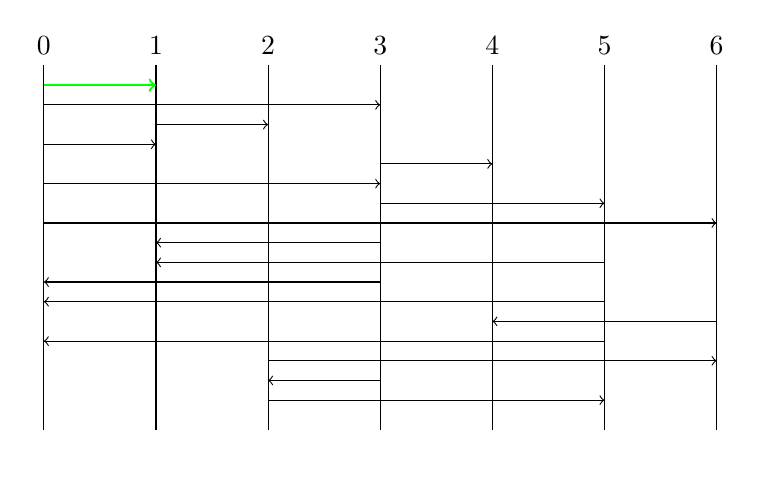
\begin{tikzpicture}
 	 					\node[] (n0) {0};
 	 					\node[right = of n0] (n1) {1};
 	 					\node[right = of n1] (n2) {2};
 	 					\node[right = of n2] (n3) {3};
 	 					\node[right = of n3] (n4) {4};
 	 					\node[right = of n4] (n5) {5};
 	 					\node[right = of n5] (n6) {6};
 	 					\node[below of=n0, node distance=5cm] (n0Ground) {};
 	 					\node[below of=n1, node distance=5cm] (n1Ground) {};
 	 					\node[below of=n2, node distance=5cm] (n2Ground) {};
 	 					\node[below of=n3, node distance=5cm] (n3Ground) {};
 	 					\node[below of=n4, node distance=5cm] (n4Ground) {};
 	 					\node[below of=n5, node distance=5cm] (n5Ground) {};
 	 					\node[below of=n6, node distance=5cm] (n6Ground) {};
 	 					% lines down
 	 					\draw (n0) -- (n0Ground);
 	 					\draw (n1) -- (n1Ground);
 	 					\draw (n2) -- (n2Ground);
 	 					\draw (n3) -- (n3Ground);
 	 					\draw (n4) -- (n4Ground);
 	 					\draw (n5) -- (n5Ground);
 	 					\draw (n6) -- (n6Ground);
 	 					%arrows
 	 					\draw[->,thick,color=green] ($(n0)!0.10!(n0Ground)$)--($(n1)!0.10!(n1Ground)$);
 	 					\draw[->] ($(n0)!0.15!(n0Ground)$)--($(n3)!0.15!(n3Ground)$);
 	 					\draw[->] ($(n1)!0.20!(n1Ground)$)--($(n2)!0.20!(n2Ground)$);
 	 					\draw[->] ($(n0)!0.25!(n0Ground)$)--($(n1)!0.25!(n1Ground)$);
 	 					\draw[->] ($(n3)!0.30!(n3Ground)$)--($(n4)!0.30!(n4Ground)$);
 	 					\draw[->] ($(n0)!0.35!(n0Ground)$)--($(n3)!0.35!(n3Ground)$);
 	 					\draw[->] ($(n3)!0.40!(n3Ground)$)--($(n5)!0.40!(n5Ground)$);
 	 					\draw[->] ($(n0)!0.45!(n0Ground)$)--($(n6)!0.45!(n6Ground)$);
 	 					\draw[->] ($(n3)!0.50!(n3Ground)$)--($(n1)!0.50!(n1Ground)$);
 	 					\draw[->] ($(n5)!0.55!(n5Ground)$)--($(n1)!0.55!(n1Ground)$);
 	 					\draw[->] ($(n3)!0.60!(n3Ground)$)--($(n0)!0.60!(n0Ground)$);
 	 					\draw[->] ($(n5)!0.65!(n5Ground)$)--($(n0)!0.65!(n0Ground)$);
 	 					\draw[->] ($(n6)!0.70!(n6Ground)$)--($(n4)!0.70!(n4Ground)$);
 	 					\draw[->] ($(n5)!0.75!(n5Ground)$)--($(n0)!0.75!(n0Ground)$);
 	 					\draw[->] ($(n2)!0.80!(n2Ground)$)--($(n6)!0.80!(n6Ground)$);
 	 					\draw[->] ($(n3)!0.85!(n3Ground)$)--($(n2)!0.85!(n2Ground)$);
 	 					\draw[->] ($(n2)!0.90!(n2Ground)$)--($(n5)!0.90!(n5Ground)$);
 	 				\end{tikzpicture}
 	 			};
 	 			\node (2) at ($(a)+(1*180/5:17cm) $) [child] {
 	 				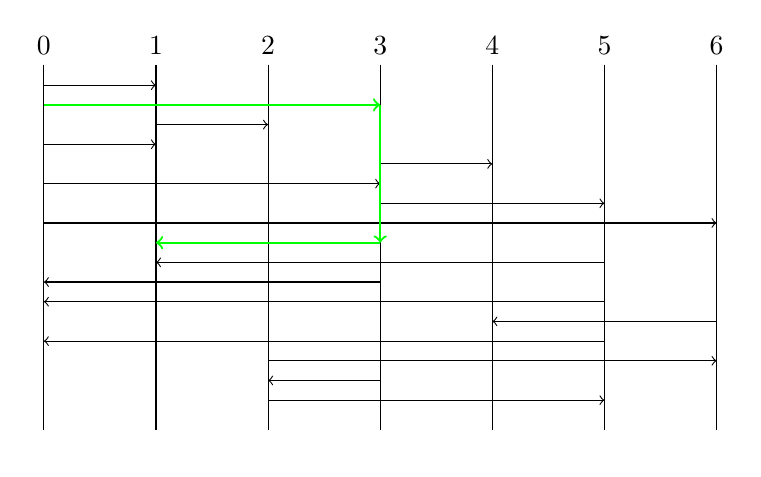
\begin{tikzpicture}
 	 					5			\node[] (n0) {0};
 	 					\node[right = of n0] (n1) {1};
 	 					\node[right = of n1] (n2) {2};
 	 					\node[right = of n2] (n3) {3};
 	 					\node[right = of n3] (n4) {4};
 	 					\node[right = of n4] (n5) {5};
 	 					\node[right = of n5] (n6) {6};
 	 					\node[below of=n0, node distance=5cm] (n0Ground) {};
 	 					\node[below of=n1, node distance=5cm] (n1Ground) {};
 	 					\node[below of=n2, node distance=5cm] (n2Ground) {};
 	 					\node[below of=n3, node distance=5cm] (n3Ground) {};
 	 					\node[below of=n4, node distance=5cm] (n4Ground) {};
 	 					\node[below of=n5, node distance=5cm] (n5Ground) {};
 	 					\node[below of=n6, node distance=5cm] (n6Ground) {};
 	 					% lines down
 	 					\draw (n0) -- (n0Ground);
 	 					\draw (n1) -- (n1Ground);
 	 					\draw (n2) -- (n2Ground);
 	 					\draw (n3) -- (n3Ground);
 	 					\draw (n4) -- (n4Ground);
 	 					\draw (n5) -- (n5Ground);
 	 					\draw (n6) -- (n6Ground);
 	 					%arrows
 	 					\draw[->] ($(n0)!0.10!(n0Ground)$)--($(n1)!0.10!(n1Ground)$);
 	 					\draw[->,thick,color=green] ($(n0)!0.15!(n0Ground)$)--($(n3)!0.15!(n3Ground)$);
 	 					\draw[->] ($(n1)!0.20!(n1Ground)$)--($(n2)!0.20!(n2Ground)$);
 	 					\draw[->] ($(n0)!0.25!(n0Ground)$)--($(n1)!0.25!(n1Ground)$);
 	 					\draw[->] ($(n3)!0.30!(n3Ground)$)--($(n4)!0.30!(n4Ground)$);
 	 					\draw[->] ($(n0)!0.35!(n0Ground)$)--($(n3)!0.35!(n3Ground)$);
 	 					\draw[->] ($(n3)!0.40!(n3Ground)$)--($(n5)!0.40!(n5Ground)$);
 	 					\draw[->] ($(n0)!0.45!(n0Ground)$)--($(n6)!0.45!(n6Ground)$);
 	 					\draw[->,thick,color=green] ($(n3)!0.50!(n3Ground)$)--($(n1)!0.50!(n1Ground)$);
 	 					\draw[->] ($(n5)!0.55!(n5Ground)$)--($(n1)!0.55!(n1Ground)$);
 	 					\draw[->] ($(n3)!0.60!(n3Ground)$)--($(n0)!0.60!(n0Ground)$);
 	 					\draw[->] ($(n5)!0.65!(n5Ground)$)--($(n0)!0.65!(n0Ground)$);
 	 					\draw[->] ($(n6)!0.70!(n6Ground)$)--($(n4)!0.70!(n4Ground)$);
 	 					\draw[->] ($(n5)!0.75!(n5Ground)$)--($(n0)!0.75!(n0Ground)$);
 	 					\draw[->] ($(n2)!0.80!(n2Ground)$)--($(n6)!0.80!(n6Ground)$);
 	 					\draw[->] ($(n3)!0.85!(n3Ground)$)--($(n2)!0.85!(n2Ground)$);
 	 					\draw[->] ($(n2)!0.90!(n2Ground)$)--($(n5)!0.90!(n5Ground)$);
 	 					% addon arrows
 	 					\draw[->,thick,color=green] ($(n3)!0.15!(n3Ground)$)--($(n3)!0.50!(n3Ground)$);
 	 				\end{tikzpicture}
 	 			};
 	 			\node (3) at ($(a)+(2*180/5:17cm) $) [child] {
 	 				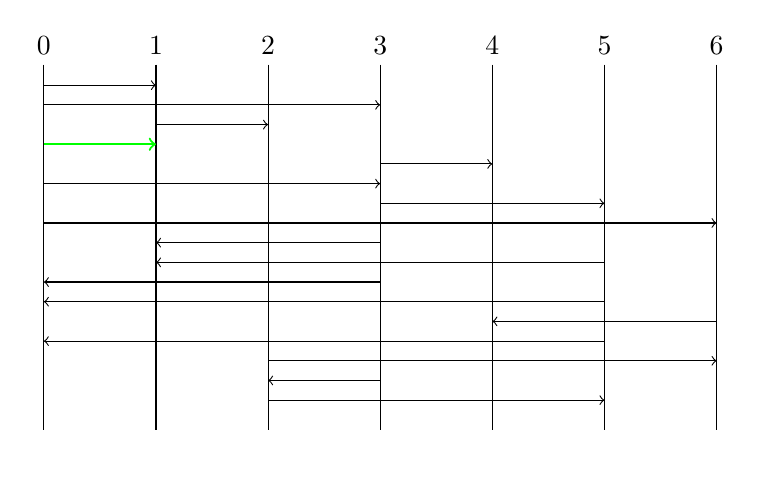
\begin{tikzpicture}
 	 					\node[] (n0) {0};
 	 					\node[right = of n0] (n1) {1};
 	 					\node[right = of n1] (n2) {2};
 	 					\node[right = of n2] (n3) {3};
 	 					\node[right = of n3] (n4) {4};
 	 					\node[right = of n4] (n5) {5};
 	 					\node[right = of n5] (n6) {6};
 	 					\node[below of=n0, node distance=5cm] (n0Ground) {};
 	 					\node[below of=n1, node distance=5cm] (n1Ground) {};
 	 					\node[below of=n2, node distance=5cm] (n2Ground) {};
 	 					\node[below of=n3, node distance=5cm] (n3Ground) {};
 	 					\node[below of=n4, node distance=5cm] (n4Ground) {};
 	 					\node[below of=n5, node distance=5cm] (n5Ground) {};
 	 					\node[below of=n6, node distance=5cm] (n6Ground) {};
 	 					% lines down
 	 					\draw (n0) -- (n0Ground);
 	 					\draw (n1) -- (n1Ground);
 	 					\draw (n2) -- (n2Ground);
 	 					\draw (n3) -- (n3Ground);
 	 					\draw (n4) -- (n4Ground);
 	 					\draw (n5) -- (n5Ground);
 	 					\draw (n6) -- (n6Ground);
 	 					%arrows
 	 					\draw[->] ($(n0)!0.10!(n0Ground)$)--($(n1)!0.10!(n1Ground)$);
 	 					\draw[->] ($(n0)!0.15!(n0Ground)$)--($(n3)!0.15!(n3Ground)$);
 	 					\draw[->] ($(n1)!0.20!(n1Ground)$)--($(n2)!0.20!(n2Ground)$);
 	 					\draw[->,thick,color=green] ($(n0)!0.25!(n0Ground)$)--($(n1)!0.25!(n1Ground)$);
 	 					\draw[->] ($(n3)!0.30!(n3Ground)$)--($(n4)!0.30!(n4Ground)$);
 	 					\draw[->] ($(n0)!0.35!(n0Ground)$)--($(n3)!0.35!(n3Ground)$);
 	 					\draw[->] ($(n3)!0.40!(n3Ground)$)--($(n5)!0.40!(n5Ground)$);
 	 					\draw[->] ($(n0)!0.45!(n0Ground)$)--($(n6)!0.45!(n6Ground)$);
 	 					\draw[->] ($(n3)!0.50!(n3Ground)$)--($(n1)!0.50!(n1Ground)$);
 	 					\draw[->] ($(n5)!0.55!(n5Ground)$)--($(n1)!0.55!(n1Ground)$);
 	 					\draw[->] ($(n3)!0.60!(n3Ground)$)--($(n0)!0.60!(n0Ground)$);
 	 					\draw[->] ($(n5)!0.65!(n5Ground)$)--($(n0)!0.65!(n0Ground)$);
 	 					\draw[->] ($(n6)!0.70!(n6Ground)$)--($(n4)!0.70!(n4Ground)$);
 	 					\draw[->] ($(n5)!0.75!(n5Ground)$)--($(n0)!0.75!(n0Ground)$);
 	 					\draw[->] ($(n2)!0.80!(n2Ground)$)--($(n6)!0.80!(n6Ground)$);
 	 					\draw[->] ($(n3)!0.85!(n3Ground)$)--($(n2)!0.85!(n2Ground)$);
 	 					\draw[->] ($(n2)!0.90!(n2Ground)$)--($(n5)!0.90!(n5Ground)$);
 	 					% addon arrows
 	 					%\draw[->,thick,color=green] ($(n3)!0.15!(n3Ground)$)--($(n3)!0.50!(n3Ground)$);
 	 				\end{tikzpicture}
 	 			};
 	 			\node (4) at ($(a)+(3*180/5:17cm) $) [child] {
 	 				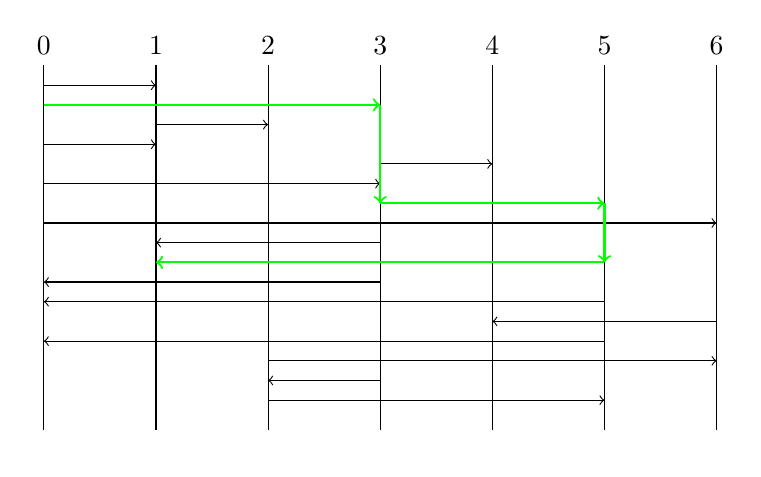
\begin{tikzpicture}
 	 					\node[] (n0) {0};
 	 					\node[right = of n0] (n1) {1};
 	 					\node[right = of n1] (n2) {2};
 	 					\node[right = of n2] (n3) {3};
 	 					\node[right = of n3] (n4) {4};
 	 					\node[right = of n4] (n5) {5};
 	 					\node[right = of n5] (n6) {6};
 	 					\node[below of=n0, node distance=5cm] (n0Ground) {};
 	 					\node[below of=n1, node distance=5cm] (n1Ground) {};
 	 					\node[below of=n2, node distance=5cm] (n2Ground) {};
 	 					\node[below of=n3, node distance=5cm] (n3Ground) {};
 	 					\node[below of=n4, node distance=5cm] (n4Ground) {};
 	 					\node[below of=n5, node distance=5cm] (n5Ground) {};
 	 					\node[below of=n6, node distance=5cm] (n6Ground) {};
 	 					% lines down
 	 					\draw (n0) -- (n0Ground);
 	 					\draw (n1) -- (n1Ground);
 	 					\draw (n2) -- (n2Ground);
 	 					\draw (n3) -- (n3Ground);
 	 					\draw (n4) -- (n4Ground);
 	 					\draw (n5) -- (n5Ground);
 	 					\draw (n6) -- (n6Ground);
 	 					%arrows
 	 					\draw[->] ($(n0)!0.10!(n0Ground)$)--($(n1)!0.10!(n1Ground)$);
 	 					\draw[->,thick,color=green] ($(n0)!0.15!(n0Ground)$)--($(n3)!0.15!(n3Ground)$);
 	 					\draw[->] ($(n1)!0.20!(n1Ground)$)--($(n2)!0.20!(n2Ground)$);
 	 					\draw[->] ($(n0)!0.25!(n0Ground)$)--($(n1)!0.25!(n1Ground)$);
 	 					\draw[->] ($(n3)!0.30!(n3Ground)$)--($(n4)!0.30!(n4Ground)$);
 	 					\draw[->] ($(n0)!0.35!(n0Ground)$)--($(n3)!0.35!(n3Ground)$);
 	 					\draw[->,thick,color=green] ($(n3)!0.40!(n3Ground)$)--($(n5)!0.40!(n5Ground)$);
 	 					\draw[->] ($(n0)!0.45!(n0Ground)$)--($(n6)!0.45!(n6Ground)$);
 	 					\draw[->] ($(n3)!0.50!(n3Ground)$)--($(n1)!0.50!(n1Ground)$);
 	 					\draw[->,thick,color=green] ($(n5)!0.55!(n5Ground)$)--($(n1)!0.55!(n1Ground)$);
 	 					\draw[->] ($(n3)!0.60!(n3Ground)$)--($(n0)!0.60!(n0Ground)$);
 	 					\draw[->] ($(n5)!0.65!(n5Ground)$)--($(n0)!0.65!(n0Ground)$);
 	 					\draw[->] ($(n6)!0.70!(n6Ground)$)--($(n4)!0.70!(n4Ground)$);
 	 					\draw[->] ($(n5)!0.75!(n5Ground)$)--($(n0)!0.75!(n0Ground)$);
 	 					\draw[->] ($(n2)!0.80!(n2Ground)$)--($(n6)!0.80!(n6Ground)$);
 	 					\draw[->] ($(n3)!0.85!(n3Ground)$)--($(n2)!0.85!(n2Ground)$);
 	 					\draw[->] ($(n2)!0.90!(n2Ground)$)--($(n5)!0.90!(n5Ground)$);
 	 					% addon arrows
 	 					\draw[->,thick,color=green] ($(n3)!0.15!(n3Ground)$)--($(n3)!0.40!(n3Ground)$);
 	 					\draw[->,thick,color=green] ($(n5)!0.40!(n5Ground)$)--($(n5)!0.55!(n5Ground)$);
 	 				\end{tikzpicture}
 	 			};
 	 			\node (5) at ($(a)+(4*180/5:17cm) $) [child] {
 	 				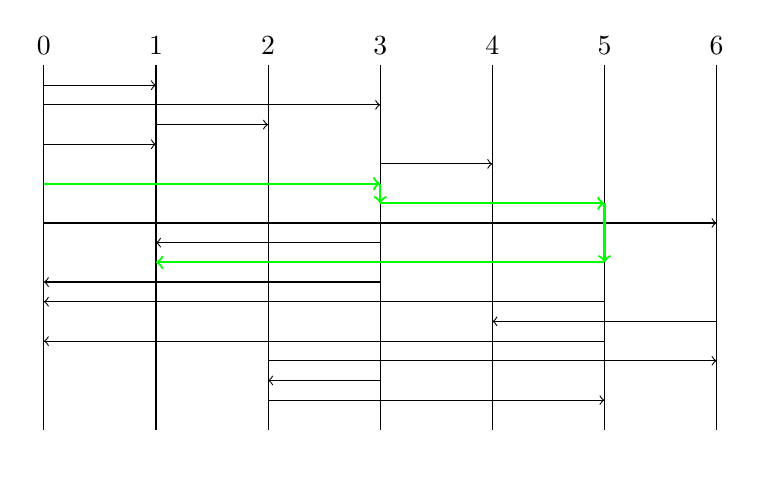
\begin{tikzpicture}
 	 					\node[] (n0) {0};
 	 					\node[right = of n0] (n1) {1};
 	 					\node[right = of n1] (n2) {2};
 	 					\node[right = of n2] (n3) {3};
 	 					\node[right = of n3] (n4) {4};
 	 					\node[right = of n4] (n5) {5};
 	 					\node[right = of n5] (n6) {6};
 	 					\node[below of=n0, node distance=5cm] (n0Ground) {};
 	 					\node[below of=n1, node distance=5cm] (n1Ground) {};
 	 					\node[below of=n2, node distance=5cm] (n2Ground) {};
 	 					\node[below of=n3, node distance=5cm] (n3Ground) {};
 	 					\node[below of=n4, node distance=5cm] (n4Ground) {};
 	 					\node[below of=n5, node distance=5cm] (n5Ground) {};
 	 					\node[below of=n6, node distance=5cm] (n6Ground) {};
 	 					% lines down
 	 					\draw (n0) -- (n0Ground);
 	 					\draw (n1) -- (n1Ground);
 	 					\draw (n2) -- (n2Ground);
 	 					\draw (n3) -- (n3Ground);
 	 					\draw (n4) -- (n4Ground);
 	 					\draw (n5) -- (n5Ground);
 	 					\draw (n6) -- (n6Ground);
 	 					%arrows
 	 					\draw[->] ($(n0)!0.10!(n0Ground)$)--($(n1)!0.10!(n1Ground)$);
 	 					\draw[->] ($(n0)!0.15!(n0Ground)$)--($(n3)!0.15!(n3Ground)$);
 	 					\draw[->] ($(n1)!0.20!(n1Ground)$)--($(n2)!0.20!(n2Ground)$);
 	 					\draw[->] ($(n0)!0.25!(n0Ground)$)--($(n1)!0.25!(n1Ground)$);
 	 					\draw[->] ($(n3)!0.30!(n3Ground)$)--($(n4)!0.30!(n4Ground)$);
 	 					\draw[->,thick,color=green] ($(n0)!0.35!(n0Ground)$)--($(n3)!0.35!(n3Ground)$);
 	 					\draw[->,thick,color=green] ($(n3)!0.40!(n3Ground)$)--($(n5)!0.40!(n5Ground)$);
 	 					\draw[->] ($(n0)!0.45!(n0Ground)$)--($(n6)!0.45!(n6Ground)$);
 	 					\draw[->] ($(n3)!0.50!(n3Ground)$)--($(n1)!0.50!(n1Ground)$);
 	 					\draw[->,thick,color=green] ($(n5)!0.55!(n5Ground)$)--($(n1)!0.55!(n1Ground)$);
 	 					\draw[->] ($(n3)!0.60!(n3Ground)$)--($(n0)!0.60!(n0Ground)$);
 	 					\draw[->] ($(n5)!0.65!(n5Ground)$)--($(n0)!0.65!(n0Ground)$);
 	 					\draw[->] ($(n6)!0.70!(n6Ground)$)--($(n4)!0.70!(n4Ground)$);
 	 					\draw[->] ($(n5)!0.75!(n5Ground)$)--($(n0)!0.75!(n0Ground)$);
 	 					\draw[->] ($(n2)!0.80!(n2Ground)$)--($(n6)!0.80!(n6Ground)$);
 	 					\draw[->] ($(n3)!0.85!(n3Ground)$)--($(n2)!0.85!(n2Ground)$);
 	 					\draw[->] ($(n2)!0.90!(n2Ground)$)--($(n5)!0.90!(n5Ground)$);
 	 					% addon arrows
 	 					\draw[->,thick,color=green] ($(n3)!0.35!(n3Ground)$)--($(n3)!0.40!(n3Ground)$);
 	 					\draw[->,thick,color=green] ($(n5)!0.40!(n5Ground)$)--($(n5)!0.55!(n5Ground)$);
 	 				\end{tikzpicture}
 	 			};
 	 			\node (6) at ($(a)+(5*180/5:17cm) $) [child] {
 	 				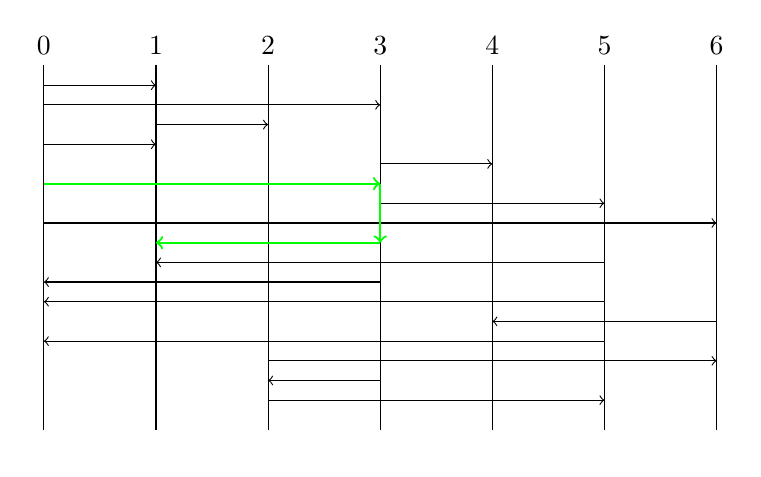
\begin{tikzpicture}
 	 					\node[] (n0) {0};
 	 					\node[right = of n0] (n1) {1};
 	 					\node[right = of n1] (n2) {2};
 	 					\node[right = of n2] (n3) {3};
 	 					\node[right = of n3] (n4) {4};
 	 					\node[right = of n4] (n5) {5};
 	 					\node[right = of n5] (n6) {6};
 	 					\node[below of=n0, node distance=5cm] (n0Ground) {};
 	 					\node[below of=n1, node distance=5cm] (n1Ground) {};
 	 					\node[below of=n2, node distance=5cm] (n2Ground) {};
 	 					\node[below of=n3, node distance=5cm] (n3Ground) {};
 	 					\node[below of=n4, node distance=5cm] (n4Ground) {};
 	 					\node[below of=n5, node distance=5cm] (n5Ground) {};
 	 					\node[below of=n6, node distance=5cm] (n6Ground) {};
 	 					% lines down
 	 					\draw (n0) -- (n0Ground);
 	 					\draw (n1) -- (n1Ground);
 	 					\draw (n2) -- (n2Ground);
 	 					\draw (n3) -- (n3Ground);
 	 					\draw (n4) -- (n4Ground);
 	 					\draw (n5) -- (n5Ground);
 	 					\draw (n6) -- (n6Ground);
 	 					%arrows
 	 					\draw[->] ($(n0)!0.10!(n0Ground)$)--($(n1)!0.10!(n1Ground)$);
 	 					\draw[->] ($(n0)!0.15!(n0Ground)$)--($(n3)!0.15!(n3Ground)$);
 	 					\draw[->] ($(n1)!0.20!(n1Ground)$)--($(n2)!0.20!(n2Ground)$);
 	 					\draw[->] ($(n0)!0.25!(n0Ground)$)--($(n1)!0.25!(n1Ground)$);
 	 					\draw[->] ($(n3)!0.30!(n3Ground)$)--($(n4)!0.30!(n4Ground)$);
 	 					\draw[->,thick,color=green] ($(n0)!0.35!(n0Ground)$)--($(n3)!0.35!(n3Ground)$);
 	 					\draw[->] ($(n3)!0.40!(n3Ground)$)--($(n5)!0.40!(n5Ground)$);
 	 					\draw[->] ($(n0)!0.45!(n0Ground)$)--($(n6)!0.45!(n6Ground)$);
 	 					\draw[->,thick,color=green] ($(n3)!0.50!(n3Ground)$)--($(n1)!0.50!(n1Ground)$);
 	 					\draw[->] ($(n5)!0.55!(n5Ground)$)--($(n1)!0.55!(n1Ground)$);
 	 					\draw[->] ($(n3)!0.60!(n3Ground)$)--($(n0)!0.60!(n0Ground)$);
 	 					\draw[->] ($(n5)!0.65!(n5Ground)$)--($(n0)!0.65!(n0Ground)$);
 	 					\draw[->] ($(n6)!0.70!(n6Ground)$)--($(n4)!0.70!(n4Ground)$);
 	 					\draw[->] ($(n5)!0.75!(n5Ground)$)--($(n0)!0.75!(n0Ground)$);
 	 					\draw[->] ($(n2)!0.80!(n2Ground)$)--($(n6)!0.80!(n6Ground)$);
 	 					\draw[->] ($(n3)!0.85!(n3Ground)$)--($(n2)!0.85!(n2Ground)$);
 	 					\draw[->] ($(n2)!0.90!(n2Ground)$)--($(n5)!0.90!(n5Ground)$);
 	 					% addon arrows
 	 					\draw[->,thick,color=green] ($(n3)!0.35!(n3Ground)$)--($(n3)!0.50!(n3Ground)$);
 	 				\end{tikzpicture}
 	 			};
 	 			
 	 			\draw[->,shorten <=25pt,shorten >=10pt,draw=red,thick] (a)--(1) node[midway,sloped,above] {path 1};
 	 			\draw[->,shorten <=25pt,shorten >=10pt,draw=red,thick] (a)--(2) node[midway,sloped,above] {path 2};
 	 			\draw[->,shorten <=25pt,shorten >=10pt,draw=red,thick] (a)--(3) node[midway,sloped,above] {path 3};
 	 			\draw[->,shorten <=25pt,shorten >=10pt,draw=red,thick] (a)--(4) node[midway,sloped,above] {path 4};
 	 			\draw[->,shorten <=25pt,shorten >=10pt,draw=red,thick] (a)--(5) node[midway,sloped,above] {path 5};
 	 			\draw[->,shorten <=25pt,shorten >=10pt,draw=red,thick] (a)--(6) node[midway,sloped,above] {path 6};
 	 			
 	 		\end{tikzpicture}
 	 	}
 	 	\caption{A graph containing six paths between node $0$ and node $1$}\label{fig:graphPaths}
 	 \end{figure}
	
	\begin{figure}[H]
	  	\centering
	  	\begin{tikzpicture}
	  		\begin{axis}[ytick={0,1088527},yticklabels={0,max},xtick={70,90,120,200},xticklabels={$70$,$90$,$120$,$200$}]
	  			\addplot[smooth] coordinates {
	  				(70,0)(71,0)(72,0)(73,0)(74,0)(75,0)(76,0)(77,0)(78,0)(79,0)
	  				(80,0)(81,0)(82,0)(83,0)(84,0)(85,0)(86,0)(87,0)(88,0)(89,0)(90,5)(91,17)(92,31)(93,63)(94,127)(95,284)(96,521)(97,1007)(98,1861)(99,3179)
	  				(100,5499)(101,9454)(102,15517)(103,25184)(104,38892)(105,59401)(106,86779)(107,124609)(108,173778)(109,236005)(110,310038)(111,398844)(112,499226)(113,606437)(114,713662)(115,820144)(116,918162)(117,995665)(118,1054089)(119,1081792)
	  				(120,1088527)(121,1082042)(122,1076051)(123,1063208)(124,1044725)(125,1025394)(126,1001131)(127,974837)(128,944276)(129,912184)(130,877056)(131,841599)(132,801819)(133,761560)(134,722383)(135,680702)(136,638947)(137,598466)(138,556899)(139,518323)
	  				(140,479028)(141,441472)(142,404478)(143,369047)(144,336823)(145,305905)(146,276225)(147,248062)(148,223072)(149,198637)(150,176465)(151,157067)(152,138213)(153,121287)(154,106923)(155,93143)(156,80291)(157,70019)(158,60285)(159,52003)
	  				(160,44159)(161,37625)(162,32157)(163,26929)(164,22780)(165,19184)(166,16166)(167,13179)(168,11125)(169,9137)(170,7434)(171,6295)(172,4924)(173,4037)(174,3300)(175,2651)(176,2092)(177,1693)(178,1367)(179,1102)
	  				(180,853)(181,687)(182,527)(183,387)(184,319)(185,241)(186,204)(187,141)(188,120)(189,99)(190,76)(191,47)(192,41)(193,19)(194,13)(195,16)(196,15)(197,6)(198,5)(199,2)
	  			};
	  		\end{axis}
	  	\end{tikzpicture}
	  	\caption{Distribution of setRandomTime(90, 120, 200)}
	  	\label{fig:timeDistribution}
	\end{figure}
	\cref{fig:timeDistribution} is a simple curve showing the distribution of an adapted probability function. This image is just the bare minimum and should look maybe a bit more professional.
  
  	\section{Part 7}
	\begin{figure}[H]
	  	\includegraphics[width=\textwidth]{inc/statanalysis_graph}
	  	\caption{Distribution Analysis of Different, Common Graphics Formats}
	  	\label{fig:statGraph}
	\end{figure}
	The graph in \cref{fig:statGraph} is for completness only listed here and maybe not sensible to recreate.
	  
	\begin{figure}[H]
	  	\includegraphics[width=\textwidth]{inc/statanalysis_mv}
	  	\caption{Distribution Analysis of a MessageVortex Block}
	  	\label{fig:statMvGraph}
	\end{figure}
	The graph in \cref{fig:statMvGraph} is for completness only listed here and maybe not sensible to recreate.

	\begin{figure}[H]\centering
		\includegraphics[width=1\textwidth]{inc/randomblock_10kb}
		\caption{Resulting entropy of addRedundancy with and without encryption step}
		\label{fig:entropy}
	\end{figure}
	The graph in \cref{fig:entropy} is for completness only listed here and maybe not sensible to recreate.

	\begin{figure}[H]\centering
		\includegraphics[width=1\textwidth]{inc/messageGraphPaths}
		\caption{A randomly generated graph with highlighted paths to the target.}
		\label{fig:messageGraphPaths}
	\end{figure}
    The graph in \cref{fig:messageGraphPaths} show how different paths in a graph offer different paths from a source to a target.


	\begin{figure}[H]\centering
		\includegraphics[width=1\textwidth]{inc/reducedMessageGraphPaths}
		\caption{A randomly generated graph assuming that all nodes except node 0 and 1 are collaborating.}
		\label{fig:reducedMessageGraphPaths}
	\end{figure}
	The graph in \cref{fig:reducedMessageGraphPaths} shows how a graph may be collapsed under worst case assumptions. This is the new representation of \cref{fig:graphPaths}. Blue boxes show nodes.
	

	\begin{figure}[!h]
		\centering\includegraphics[width=0.7\columnwidth]{inc/messagePaths}
		\caption{A possible path of a VortexMessage}
		\label{fig:messagePaths}
	\end{figure}
    I am very unhappy with the visualization in figure \cref{fig:messagePaths}. The graphics looks too simple, lacks a legend and nodes look dull/stupid. Somehow they should be a small representation of the three layers of \cref{fig:protocolLayers}.
	
	\begin{figure}[H]\centering
		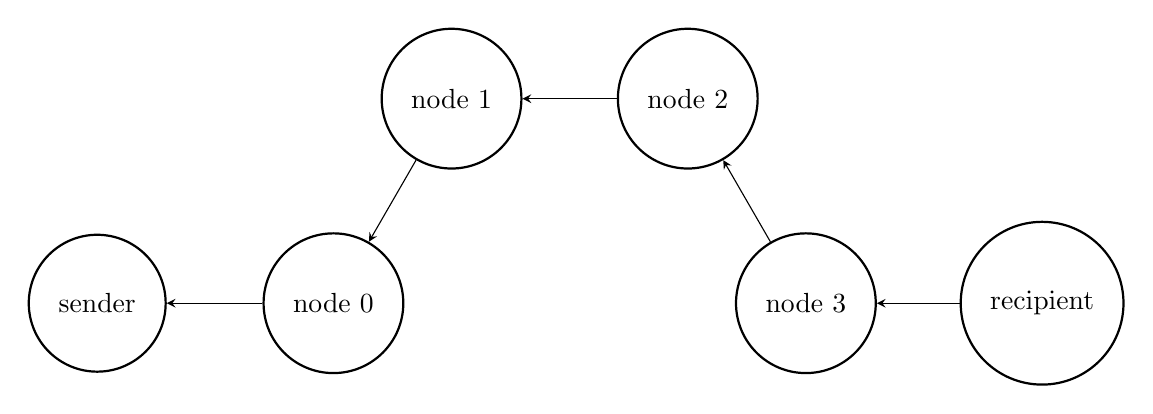
\begin{tikzpicture}[node distance=0.5cm,auto,>=stealth]
			\begin{scope}[baseline=(current bounding box.center)]
				\tikzstyle{knode}=[circle,draw=black,thick,inner sep=8pt,baseline=(current bounding box.center)]
				\node[knode] (n-1) at (0:6cm) {recipient};
				\node[knode] (n0) at (0:3cm) {node 3};
				\node[knode] (n1) at (60:3cm) {node 2};
				\node[knode] (n2) at (120:3cm) {node 1};
				\node[knode] (n3) at (180:3cm) {node 0};
				\node[knode] (n4) at (180:6cm) {sender};
				%arrows
				\draw[->] (n-1)--(n0);
				\draw[->] (n0)--(n1);
				\draw[->] (n1)--(n2);
				\draw[->] (n2)--(n3);
				\draw[->] (n3)--(n4);
			\end{scope}
		\end{tikzpicture}
		\caption{A typical Mixminion mix cascade}
		\label{fig:mmCommPattern}
	\end{figure}
	
	\begin{figure}[H]\centering
		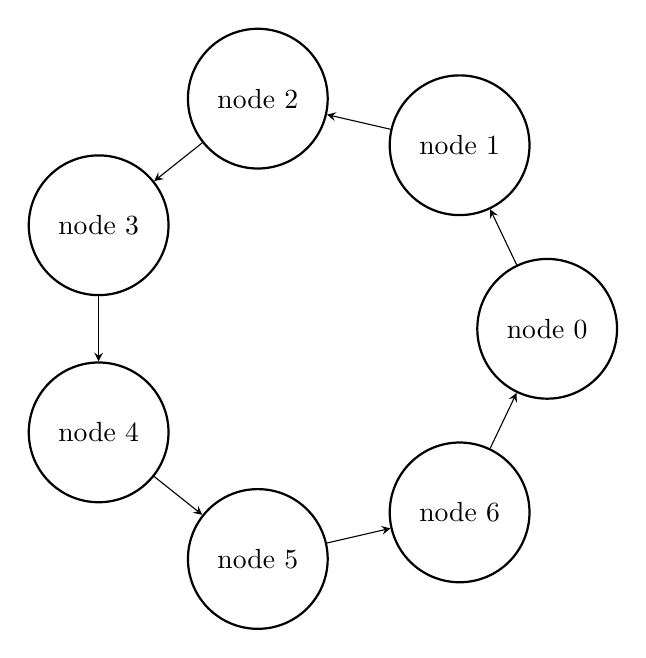
\begin{tikzpicture}[node distance=0.5cm,auto,>=stealth]
			\begin{scope}[baseline=(current bounding box.center)]
				\tikzstyle{knode}=[circle,draw=black,thick,inner sep=8pt,baseline=(current bounding box.center)]
				\node[knode] (n0) at (0:3cm) {node 0};
				\node[knode] (n1) at (51:3cm) {node 1};
				\node[knode] (n2) at (103:3cm) {node 2};
				\node[knode] (n3) at (154:3cm) {node 3};
				\node[knode] (n4) at (206:3cm) {node 4};
				\node[knode] (n5) at (257:3cm) {node 5};
				\node[knode] (n6) at (309:3cm) {node 6};
				%arrows
				\draw[->] (n0)--(n1);
				\draw[->] (n1)--(n2);
				\draw[->] (n2)--(n3);
				\draw[->] (n3)--(n4);
				\draw[->] (n4)--(n5);
				\draw[->] (n5)--(n6);
				\draw[->] (n6)--(n0);
			\end{scope}
		\end{tikzpicture}
		\caption{A typical DC network communication pattern}
		\label{fig:dcCommPattern}
	\end{figure}

	\begin{figure}[H]\centering
		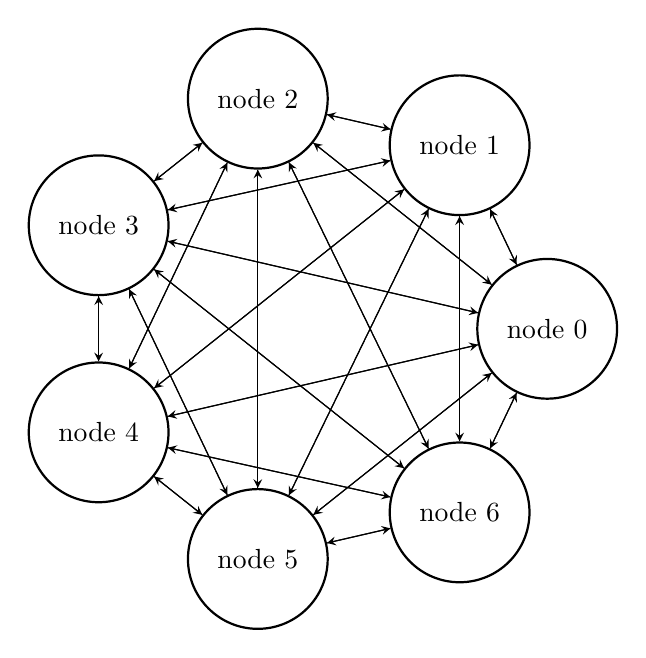
\begin{tikzpicture}[node distance=0.5cm,auto,>=stealth]
			\begin{scope}[baseline=(current bounding box.center)]
				\tikzstyle{knode}=[circle,draw=black,thick,inner sep=8pt,baseline=(current bounding box.center)]
				\node[knode] (n0) at (0:3cm) {node 0};
				\node[knode] (n1) at (51:3cm) {node 1};
				\node[knode] (n2) at (103:3cm) {node 2};
				\node[knode] (n3) at (154:3cm) {node 3};
				\node[knode] (n4) at (206:3cm) {node 4};
				\node[knode] (n5) at (257:3cm) {node 5};
				\node[knode] (n6) at (309:3cm) {node 6};
				%arrows
				\draw[->] (n0)--(n1);
				\draw[->] (n0)--(n2);
				\draw[->] (n0)--(n3);
				\draw[->] (n0)--(n4);
				\draw[->] (n0)--(n5);
				\draw[->] (n0)--(n6);
				\draw[->] (n1)--(n0);
				\draw[->] (n1)--(n2);
				\draw[->] (n1)--(n3);
				\draw[->] (n1)--(n4);
				\draw[->] (n1)--(n5);
				\draw[->] (n1)--(n6);
				\draw[->] (n2)--(n0);
				\draw[->] (n2)--(n1);
				\draw[->] (n2)--(n3);
				\draw[->] (n2)--(n4);
				\draw[->] (n2)--(n5);
				\draw[->] (n2)--(n6);
				\draw[->] (n3)--(n0);
				\draw[->] (n3)--(n1);
				\draw[->] (n3)--(n2);
				\draw[->] (n3)--(n4);
				\draw[->] (n3)--(n5);
				\draw[->] (n3)--(n6);
				\draw[->] (n4)--(n0);
				\draw[->] (n4)--(n1);
				\draw[->] (n4)--(n2);
				\draw[->] (n4)--(n3);
				\draw[->] (n4)--(n5);
				\draw[->] (n4)--(n6);
				\draw[->] (n5)--(n0);
				\draw[->] (n5)--(n1);
				\draw[->] (n5)--(n2);
				\draw[->] (n5)--(n3);
				\draw[->] (n5)--(n4);
				\draw[->] (n5)--(n6);
				\draw[->] (n6)--(n0);
				\draw[->] (n6)--(n1);
				\draw[->] (n6)--(n2);
				\draw[->] (n6)--(n3);
				\draw[->] (n6)--(n4);
				\draw[->] (n6)--(n5);
			\end{scope}
		\end{tikzpicture}
		\caption{A typical broadcast network communication pattern (full mesh)}
		\label{fig:bcCommPattern}
	\end{figure}

	\begin{figure}[H]\centering
		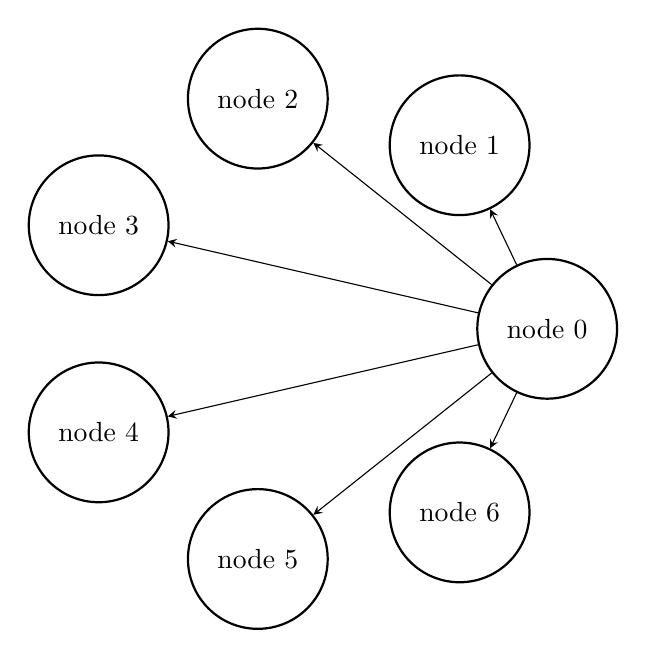
\begin{tikzpicture}[node distance=0.5cm,auto,>=stealth]
			\begin{scope}[baseline=(current bounding box.center)]
				\tikzstyle{knode}=[circle,draw=black,thick,inner sep=8pt,baseline=(current bounding box.center)]
				\node[knode] (n0) at (0:3cm) {node 0};
				\node[knode] (n1) at (51:3cm) {node 1};
				\node[knode] (n2) at (103:3cm) {node 2};
				\node[knode] (n3) at (154:3cm) {node 3};
				\node[knode] (n4) at (206:3cm) {node 4};
				\node[knode] (n5) at (257:3cm) {node 5};
				\node[knode] (n6) at (309:3cm) {node 6};
				%arrows
				\draw[->] (n0)--(n1);
				\draw[->] (n0)--(n2);
				\draw[->] (n0)--(n3);
				\draw[->] (n0)--(n4);
				\draw[->] (n0)--(n5);
				\draw[->] (n0)--(n6);
			\end{scope}
		\end{tikzpicture}
		\label{fig:bcRedCommPattern}
		\caption{A reduced broadcast network communication pattern (single broadcast)}
	\end{figure}
    The figures \ref{fig:mmCommPattern}, \ref{fig:dcCommPattern}, \ref{fig:bcCommPattern}, \ref{fig:bcRedCommPattern} look dull but okay.
    
    \section{Not in the work (but should be added again)})
    \begin{figure}[H]\centering
    	\includegraphics{inc/workspace_layout}
		\label{fig:wslayout}
		\caption{The layout of a workspace}
   	\end{figure}
    The \cref{fig:wslayout} visualizes the layout of a workspace. It contains a routing block from \cref{fig:messageOutline}, operations (e.g., \cref{fig:addRedundancyOperation}) and the workspace slots (where the payloads may be placed from \cref{fig:messageOutline}).
    
    \section{MessageVortex Text}
    {\fontfamily{lmss}\selectfont%\renewcommand{\bfdefault}{bx}\bf
     Message\includegraphics[height=1.1\fontcharht\font`V]{../../../../website/src/main/jbake/assets/images/MessageVortexLogo_huge}ortex}
	
\end{document}